\documentclass{../document}

\addbibresource{refs.bib}

\begin{document}
	\title
		[Caltech SURF First Interim Report]
		{Iago Mendes\fnote{\tt imendes@caltech.edu, ibrazmen@oberlin.edu}}
		{Control of Black Hole Parameters for Binary Evolutions}

	\section{Introduction}

  In the early twentieth century, Einstein revolutionized the study of gravity by connecting spacetime geometry with physical dynamics. As John Wheeler says, ``Spacetime tells matter how to move; matter tells spacetime how to curve'' \cite{Wheeler}. Being a highly complex theory, many problems of interest only have analytic solutions in special cases with symmetry. In this context, Numerical Relativity emerged as an essential field to solve these problems numerically, allowing us to explore general cases that can be found in the universe. Specifically, simulations of Binary Black Holes (BBH) became very important as gravitational wave detectors were developed, needing to use numerical results to identify and characterize signals in their data \cite{LIGO}.

	Famously, the Einstein equations relate the curvature of spacetime to the stress-energy of matter, forming a system of ten nonlinear partial differential equations (PDEs). With the 3+1 formalism, we can rearrange these equations so that spacetime is described by spacelike three-dimensional slices of constant time \cite{Alcubierre}. In doing so, we find that four out of the ten equations do not involve time derivatives, implying that they are constraints that must be satisfied at all times. The remaining six equations describe an evolution of the constraint-satisfying fields. Using this formalism, the Spectral Einstein Code ({\tt SpEC}) \cite{SpEC} runs BBH simulations by first finding initial data and then running an evolution on them. Over time, as {\tt SpEC} faced more challenging BBH with high mass ratios and spins, several improvements had to be made to the initial data techniques, which are summarized in \cite{Serguei}.
	
	Despite its success in BBH simulations, {\tt SpEC} shows its limitations in more challenging problems, such as binary neutron star mergers and BBH with extreme configurations. In this context, {\tt SpECTRE} \cite{SpECTRE} was created as a codebase that follows a better parallelism model and aims to be more scalable \cite{Kidder}. Previous work has already shown that {\tt SpECTRE} can be faster and more accurate than {\tt SpEC} when performing similar tasks due to its use of parallelism \cite{Vu}. This will be especially needed for the upcoming gravitational wave detectors with higher sensitivity, such as the Cosmic Explorer, the Einstein Telescope and LISA.
	
	As part of an effort to allow researchers to fully simulate BBH in {\tt SpECTRE}, an initial data procedure similar to the one in {\tt SpEC} needs to be completed. This is greatly benefitted by a scalable elliptic solver that was recently developed \cite{Vu}, which can now be used to solve the initial data equations. Be that as it may, before the start of the SURF program, {\tt SpECTRE} did not have a way to enforce specific masses and spins for the black holes or to avoid drifts in the orbital trajectory. As described in the next section, this is the problem that this research project aims to address.
  
  \section{Numerical Method}

  To find initial data, {\tt SpEC} uses the extended conformal thin-sandwich (XCTS) decomposition \cite{Serguei}, which transforms the constraint PDEs into a system of five elliptic PDEs. Before solving the XCTS equations, we need to specify the conformal spatial metric $\bar\gamma_{ij}$, the extrinsic curvature trace $K$, and their respective time derivatives $\partial_t \bar\gamma_{ij}$ and $\partial_t K$ \cite{BaumgarteShapiro}. There are many methods for specifying these quantities, but the one that has shown to be the most promising for BBH simulations is the superposed Kerr-Schild (SKS) approach \cite{Lovelace2008}. It enforces quasiequilibrium conditions by setting $\partial_t \bar\gamma_{ij}=0$ and $\partial_t K=0$. Additionally, as the name suggests, it specifies $\bar\gamma_{ij}$ and $K$ by superposing two analytic solutions of Kerr-Schild black holes with masses $M^\text{Kerr}_A$ and $M^\text{Kerr}_B$ and with dimensionless spins $\vec\chi^\text{Kerr}_A$ and $\vec\chi^\text{Kerr}_B$.

  When constructing the SKS analytical expressions for $\bar\gamma_{ij}$ and $K$, we also need to choose the centers of the black holes $\vec c_A$ and $\vec c_B$. When setting up a simulation, it is more convenient to specify their relative distance $\vec D=\vec c_A - \vec c_B$. Because of this, for any choice of $\vec c_A$, we have $\vec c_B = \vec c_A + \vec D$. In other words, we only have to choose $\vec c_A$.

  Having $\bar\gamma_{ij}$, $K$, $\partial_t \bar\gamma_{ij}$ and $\partial_t K$ specified, we can use the elliptic solver on the XCTS equations, three of which will be solved for the shift $\beta^i$. Similar to any elliptic PDE problem, we have to set boundary conditions before solving these equations. In the boundary conditions of $\vec\beta$, we can add a constant velocity $\vec v_0$, giving us more control over the initial kinematics of the binary system.

  Once the XCTS equations are solved, we have all the information that we need about the zero-time slice of spacetime. With this, we can use an apparent horizon finder to get measurements of the black holes in the constructed initial data. Let $M_A$, $M_B$, $\vec\chi_{A}$ and $\vec\chi_{B}$ be the masses and spins of the actual black holes that we have been able to create. In general, these values will differ from the ``target'' quantities $M^*_A$, $M^*_B$, $\vec\chi^*_{A}$ and $\vec\chi^*_{B}$. For example, suppose that we wish to simulate an equal-mass non-spinning case with $M^*_A = M^*_B = 0.5$ and $\vec\chi^*_{A} = \vec\chi^*_{B} = (0,0,0)$. In order to construct the SKS analytical expressions, it is natural to specify $M^\text{Kerr}_{A,B} = M^*_{A,B}$ and $\vec\chi^\text{Kerr}_{A,B} = \vec\chi^*_{A,B}$. With this, we can solve the XCTS equations and find horizons in the resulting initial data. Once we do it in {\tt SpECTRE}, we find that the resulting black hole parameters are actually $M_{A,B} \approx 0.6$ and $\vec\chi_{A,B} \approx (0,0,-0.002)$.

  If we measure other parameters of the binary, we might find that they are also not desirable. The center of mass $\vec C$ can be found by evaluating the integral
  \begin{equation} \label{eq:CoM}
    \vec C = \frac{3}{8 \pi M_\text{ADM}} \oint_{S_\infty} \psi^4 \, d\vec S,
  \end{equation}
  \cite{Serguei}, where $\psi$ is the conformal factor and $S_\infty$ is a surface at infinite radius over which we evaluate the surface integral. $M_\text{ADM}$ is the ADM mass, defined as
  \begin{equation} \label{eq:Madm}
    M_\text{ADM} = \frac{1}{16 \pi} \int_{S_\infty} \sqrt{\gamma} \gamma^{jn} \gamma^{im} (\partial_j \gamma_{mn} - \partial_m \gamma_{jn}) \, dS_j
  \end{equation}
  \cite{BaumgarteShapiro}, where $\gamma_{ij}$ is the spatial metric, $\gamma^{ij}$ is the inverse spatial metric, and $\gamma$ is the determinant of $\gamma_{ij}$. We can also use the ADM formalism to measure the total linear momentum $\vec P_\text{ADM}$ as
  \begin{equation} \label{eq:Padm}
    P_\text{ADM}^i = \frac{1}{8\pi} \oint_{S_\infty} (K^{ij} - K \gamma^{ij}) \, dS_j
  \end{equation}
  \cite{Serguei}, where $K^{ij}$ is the inverse extrinsic curvature. Ideally, $\vec C$ and $\vec P_\text{ADM}$ should be equal to zero in order to minimize any drifts of the orbit, especially for long simulations. However, similar to the example above, we can only know these quantities after the initial data has been constructed.
  
  Note that $M_{A,B}$, $\vec\chi_{A,B}$, $\vec C$ and $\vec P_\text{ADM}$ are the parameters that we wish to control, but we cannot directly set them to the desired values. The way that {\tt SpEC} handles this issue is by iterating over different choices of the free data ($M^\text{Kerr}_{A,B}$, $\vec\chi^\text{Kerr}_{A,B}$, $\vec c_A$ and $\vec v_0$), trying to find the ones that result in the ideal physical parameters. The goal of this project is to reproduce this iterative scheme in {\tt SpECTRE}. Figure \ref{fig:control-loop} shows a schematic representation of this ``control loop''.

  \begin{figure}
    \centering
    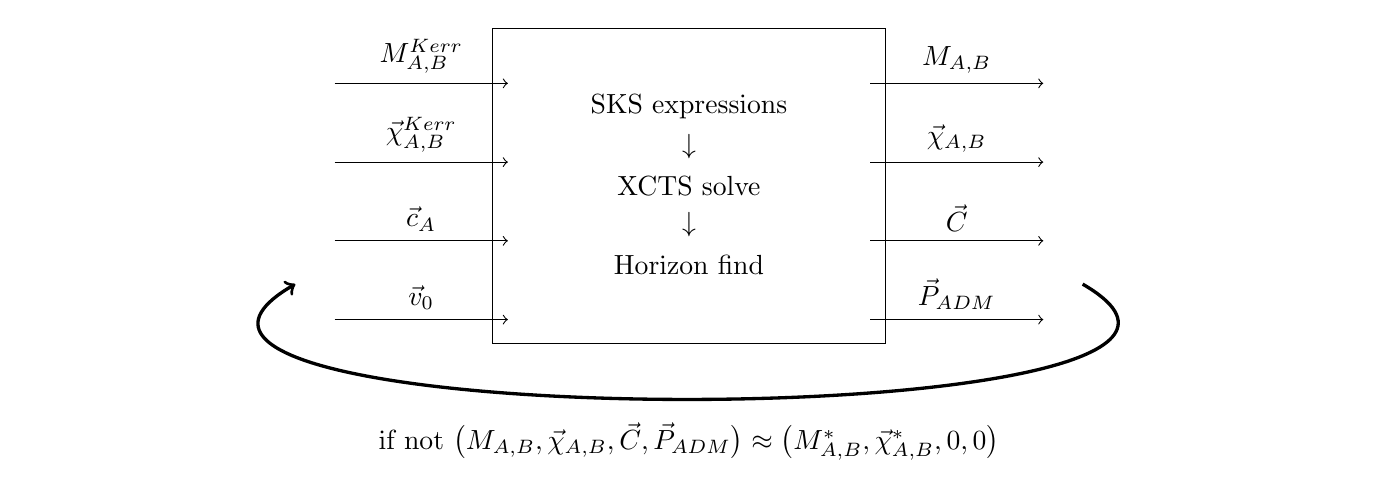
\begin{tikzpicture}
      \node at (0,+1) {SKS expressions};
      \node at (0,+0.5) {$\downarrow$};
      \node at (0,0) {XCTS solve};
      \node at (0,-0.5) {$\downarrow$};
      \node at (0,-1) {Horizon find};

      \draw (-2.5,-2) rectangle (2.5,2);

      \draw[->] (-4.5,1.3) -- (-2.3,1.3) node[anchor = south, pos = 0.5] {$M^\text{Kerr}_{A,B}$};
      \draw[->] (-4.5,0.3) -- (-2.3,0.3) node[anchor = south, pos = 0.5] {$\vec\chi^\text{Kerr}_{A,B}$};
      \draw[->] (-4.5,-0.7) -- (-2.3,-0.7) node[anchor = south, pos = 0.5] {$\vec c_A$};
      \draw[->] (-4.5,-1.7) -- (-2.3,-1.7) node[anchor = south, pos = 0.5] {$\vec v_0$};

      \draw[->] (2.3,1.3) -- (4.5,1.3) node[anchor = south, pos = 0.5] {$M_{A,B}$};
      \draw[->] (2.3,0.3) -- (4.5,0.3) node[anchor = south, pos = 0.5] {$\vec\chi_{A,B}$};
      \draw[->] (2.3,-0.7) -- (4.5,-0.7) node[anchor = south, pos = 0.5] {$\vec C$};
      \draw[->] (2.3,-1.7) -- (4.5,-1.7) node[anchor = south, pos = 0.5] {$\vec P_\text{ADM}$};

      \draw[->, very thick] (5,-1.25) to [out=-30,in=-150] (-5,-1.25);
      \node at (0,-3.25) {if not $\big(M_{A,B}, \vec\chi_{A,B}, \vec C, \vec P_\text{ADM}\big) \approx \big(M^*_{A,B}, \vec\chi^*_{A,B}, 0, 0\big)$};
    \end{tikzpicture}
    \caption{Schematic representation of the control loop.}
    \label{fig:control-loop}
  \end{figure}

  Let the choices of $M^\text{Kerr}_{A,B}$ and $\vec\chi^\text{Kerr}_{A,B}$ be represented as
  \begin{equation}
    {\bf u} = \Big( M^\text{Kerr}_A, M^\text{Kerr}_B, \chi^{\text{Kerr},x}_A, \chi^{\text{Kerr},y}_A, \chi^{\text{Kerr},z}_A, \chi^{\text{Kerr},x}_B, \chi^{\text{Kerr},y}_B, \chi^{\text{Kerr},z}_B \Big).
  \end{equation}
  Also, let the difference between the current and target physical parameters be represented as
  \begin{equation}
    \begin{aligned}
      {\bf F}({\bf u}) &= \Big( M_A - M^*_A, M_B - M^*_B, \chi^x_A - \chi^{*,x}_A, \chi^y_A - \chi^{*,y}_A, \\
      &\qquad\quad \chi^z_A - \chi^{*,z}_A, \chi^x_B - \chi^{*,x}_B, \chi^y_B - \chi^{*,y}_B, \chi^z_B - \chi^{*,z}_B \Big).
    \end{aligned}
  \end{equation}
  As discussed in the example above, it is natural to use the target parameters as an initial guess for the Kerr masses and spins:
  \begin{equation}
    {\bf u}_0 = \Big( M^*_A, M^*_B, \chi^{*,x}_A, \chi^{*,y}_A, \chi^{*,z}_A, \chi^{*,x}_B, \chi^{*,y}_B, \chi^{*,z}_B \Big).
  \end{equation}
  If we also assume that $M_{A,B}|_0 \approx M^\text{Kerr}_{A,B}|_0$ and $\vec\chi_{A,B}|_0 \approx \vec\chi^\text{Kerr}_{A,B}|_0$, then a good initial approximation for the Jacobian of ${\bf F}({\bf u})$ is $\mathbb{J}_0 \approx \mathbb{I}$ (a 8x8 identity matrix). With this, we can update our free data at every control iteration $k \geq 1$ using a Newton-Raphson scheme \cite{NumericalRecipes}:
  \begin{equation}\label{eq:u-iteration}
    {\bf u}_k = {\bf u}_{k-1} - \mathbb{J}^{-1}_{k-1} \cdot {\bf F}_{k-1}.
  \end{equation}
  Then, we can update the Jacobian with Broyden's method \cite{NumericalRecipes}:
  \begin{equation}\label{eq:J-iteration}
    \mathbb{J}_k = \mathbb{J}_{k-1} + \frac{{\bf F}_k \otimes {\bf \Delta u}_k}{||{\bf \Delta u}_k||^2},
  \end{equation}
  where we use $\Delta x_k = x_k - x_{k-1}$ for any variable $x$ from now on.

  We can also come up with iterative schemes for the choices of $\vec c_A$ and $\vec v_0$. To drive the center of mass $\vec C$ to zero we can update $\vec c_A$ as
  \begin{equation} \label{eq:cA-iteration}
		\vec c_{A,k} = \vec c_{A,k-1} - \vec C_{k-1} - \frac{M_{A,k-1}  \Delta M_{B,k-1} - M_{B,k-1} \Delta M_{A,k-1}}{(M_{A,k-1} + M_{B,k-1})^2} \vec D
  \end{equation}
  \cite{Serguei}. Considering a small perturbation of $\vec v_0$, we can drive the linear momentum $\vec P_\text{ADM}$ to zero with
  \begin{equation}\label{eq:v0-iteration}
    \begin{aligned}
      \vec v_{0,k+1} = \vec v_{0,k-1} - \frac{\vec P_{\text{ADM},k-1}}{M_{k-1}} &+ \Delta M_{k-1} (\vec v_{0,k-1} + \vec\Omega_0 \times \vec c_{A,k-1}) \\
      &- \vec\Omega_0 \times \delta \vec c_{A,k-1} - \frac{\Delta M_{B,k-1}}{M_{k-1}} \vec\Omega_0 \times \vec D
    \end{aligned}
  \end{equation}
	\cite{Serguei}, where $M_k = M_{A,k} + M_{B,k}$, $\vec \Omega_0$ is a user-specified initial orbit angle, and $\delta \vec c_{A,k}$ is a small perturbation of $\vec c_{A,k}$.

	\section{Progress Update}

  As an initial step, my co-mentor Nils Vu\fnote{nilsvu@caltech.edu} and I decided to implement the control of masses and spins as outlined in equations \eqref{eq:u-iteration} and \eqref{eq:J-iteration}. This was a good way to get used with {\tt SpECTRE} development without diving deep into its more complicated infrastructure as this was implemented in the {\tt Python} files of the codebase. We decided to differ from the approach in \cite{Serguei} in some aspects, such as using $M^\text{Kerr}_{A,B}$ and $\vec\chi^\text{Kerr}_{A,B}$ instead of the black holes radii and angular frequencies. This implementation was merged into {\tt SpECTRE}'s development branch within my first week. Since then, I have heard positive feedback from other researchers in our group who have used this feature. Figure \ref{fig:control-tests} shows some initial data configurations that were used to test this control loop.

  \begin{figure}
    \centering
    \includegraphics[width=0.8\textwidth]{assets/control_iterations_over_parameter_space.pdf}
    \caption{Tests of the current control loop over part of the parameter space of masses and spins.}
    \label{fig:control-tests}
  \end{figure}

  Next, I got started with the {\tt C++} infrastructure of {\tt SpECTRE}. With the goal of implementing a measure of the ADM total linear momentum as described in equation \eqref{eq:Padm}, I created pointwise functions to compute the integrands of such computation given the available tensors. These functions were tested with an analytic solution of a single boosted Kerr-Schild black hole. With a boost speed of $v$, we expect a linear momentum magnitude equal to
  \begin{equation}
    P_\text{expected} = \gamma M v,
  \end{equation}
  where $\gamma = 1/\sqrt{1-v^2}$ is the Lorentz factor and $M$ is the mass of the black hole. Figure \ref{fig:momentum-convergence} shows a convergence of the difference between the measured and expected linear momenta as we increase the outer boundary radius $R_\text{outer}$, over which we perform the surface integral in equation \eqref{eq:Padm}. From the convergence test, we see that this error decays as $1/R_\text{outer}$, as expected.

  \begin{figure}
    \centering
    \includegraphics[width=0.8\textwidth]{assets/adm_linear_momentum_residual_vs_distance.pdf}
    \caption{Converge test of the ADM total linear momentum computed as a surface integral.}
    \label{fig:momentum-convergence}
  \end{figure}

  After that, I started working on computing the linear momentum surface integral as part of the executable that solves the XCTS equations. This required me to learn some details of the {\tt SpECTRE} infrastructure for data boxes and parallelism. I am currently developing this feature, which should be merged within a week at most.

	\section{Future Work}

  As an immediate next step, I plan on implementing the computation of the center of mass as described in equation \eqref{eq:CoM}, which will also require me to compute the ADM mass as in equation \eqref{eq:Madm}. Both of these will involve surface integrals similar to the one used in equation \eqref{eq:Padm}, so their implementation should benefit from my previous work. Once this is done, {\tt SpECTRE} will be able to compute $\vec C$ and $\vec P_\text{ADM}$, allowing me to use equations \eqref{eq:cA-iteration} and \eqref{eq:v0-iteration} to control these quantities.

  As described in \cite{Serguei}, it is possible to use Gauss' law to split the surface integrals at infinity found in equations \eqref{eq:CoM}-\eqref{eq:Padm} into a surface integral at a smaller radius plus a volume integral. While testing the computation of $\vec P_\text{ADM}$, I briefly tried this approach, but the results were worse than evaluating the surface integral at infinity. However, this method has shown to be more numerically accurate in {\tt SpEC} \cite{Serguei}, so it is important for us to further experiment with it.

  Additionally, improvements to the control loop scheme should be made. A quick one is to re-use the previous XCTS solutions as an initial guess for the following XCTS solve. This should not reduce the number of control iterations, but it will drastically decrease the time that it takes for each iteration to run. Apart from that, we must try to test extreme configurations (high mass ratios and spins), which could potentially require adding optimizations to our current method, such as line search.

  Finally, we have been discussing novel improvements that we can make to account for the effects of junk radiation in the BBH physical parameters. Junk radiation is a collection of irregularities in the early evolution of numerical relativity simulations, which happens due to not accurately representing the past of related fields. Usually, researchers wait until junk radiation has stopped affecting the simulation and only consider the results thereafter. At that point, the physical parameters might have substantially deviated from the desired values due to the energy exchanges with such radiation. This makes it especially hard to get more extreme spins.
  
  There have been previous attempts at predicting the effects of junk radiation on the BBH masses and spins \cite{JunkRadiation}, using statistics to choose initial values that might result in the desired values after junk radiation has relaxed. Given the infrastructure that we have implemented for the initial data control loop, it would be relatively straightforward to attempt something similar. We are considering using a data-driven machine learning model, which could potentially perform better than a statistical model. We have also considered ways to mitigate junk radiation using perturbation theory, but this is a more uncertain idea.

	\section*{References}

	\printbibliography[heading=none]
\end{document}
